% !TEX root = ../main.tex

\chapter{相关工作与本文编译链概览} \label{ch:related}

如第\ref{sec:compcertbackend}节中所述,在经验证的编译器领域,许多工作是围绕CompCert编译器开展的。
我们将在第\ref{sec:relatedc}节中对CompCert及它的扩展CompCertSSA中端进行介绍。
在本章第\ref{sec:relatedf}节中,我们将对已有的针对函数式语言编译器的形式化验证工作进行介绍。
它们大部分还是基于CompCert完成的。 
国内外的研究者们已经注意到使函数式编译器复用基于SSA中间语言的基础设施后端的重要性。
在第\ref{sec:relatedssa}节中,我们对基于SSA中间语言的LLVM编译框架以及经验证的LLVM IR进行了介绍。
我们的工作基于对这些相关工作的观察建立,是朝着构建利用SSA中间语言优势的经验证的函数式编译器迈出的第一步。
我们构建了从PCF到SSA语言经验证的编译过程,并将其应用到目标语言是LLVM IR的编译链中。
在本章第~\ref{sec:overview}节中,我们对该编译链的每一步编译过程进行了简要介绍。

\section{经验证的编译器框架CompCert} \label{sec:relatedc}

经验证的C语言编译器CompCert提供了对编译器正确性进行形式化验证的理论和框架~\cite{leroy2009formally}。
它的大体编译流程如图\ref{fig:compcert}所示。该图是CompCert编译链图的简化版本,
省略了一些编译步骤,主要保留了我们在后文中介绍基于CompCert的工作时需要了解的中间语言和编译步骤。
本文中的工作所使用的基于模拟的验证技术是CompCert框架中提供的。
\begin{figure}[htbp]
    \centering
    \vspace{3ex}
    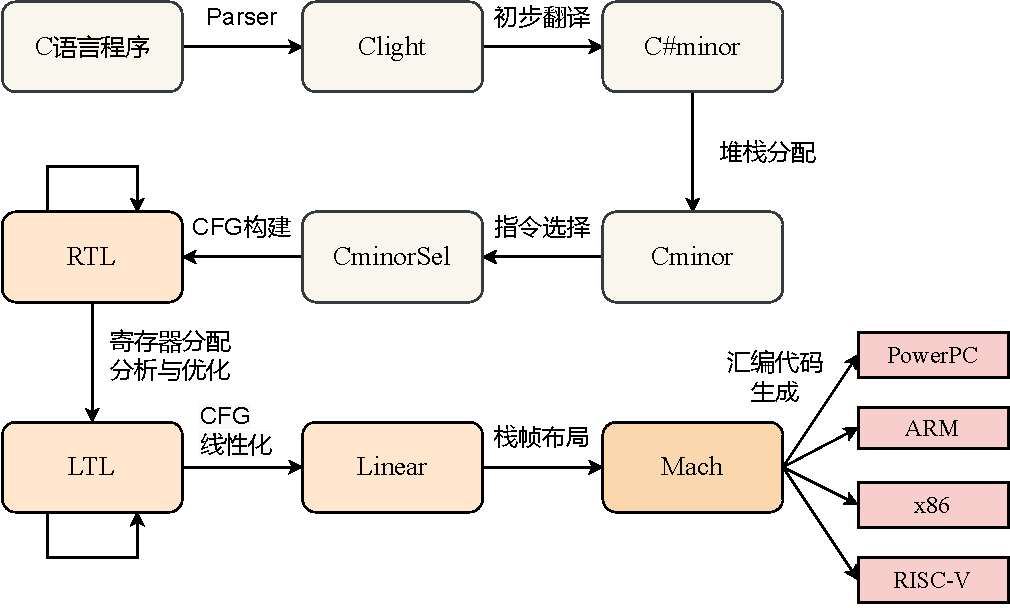
\includegraphics[width=0.8\linewidth]{figures/compcert.pdf}
    \caption{CompCert编译链概览}\label{fig:compcert}
\end{figure}

CompCertSSA是CompCert的一个扩展,具有一个基于SSA的中间端~\cite{compcertssa}。
它将SSA作为一种可选的优化中间语言,允许在RTL(Register Transfer Language)三地址代码和SSA中间语言之间进行转换。
CompCertSSA将RTL语言转换为SSA,经过全局值编号(Global Value Numbering,GVN)优化,再转换回RTL。
GVN优化是指对相同值的变量赋予相同的编号,从而消除冗余的计算。这里的SSA程序状态与RTL程序状态类似,
但是寄存器和当前函数类型要进行修改。在CompCertSSA中,$\phi$函数没有放在基本代码块中,
$\phi$指令代码块与普通指令构成的基本块是平行的结构。它们的语义也是平行定义的,
对基本代码块的控制流图定义了小步操作语义,对$\phi$指令代码块定义了大步操作语义。

虽然这使得CompCert能够实现一些基于SSA的优化~\cite{compcertssa-op,blazy-cpp2023},
但是CompCertSSA提供的优化仍然比较有限,不能与LLVM的后端优化相媲美。
本文中的SSA目标语言选择了接近LLVM中间语言的形式,也是为了对经验证的函数式语言编译器复用LLVM后端优化提供基础。
不过,它提供了一个从C语言开始的经过完整验证的编译链,是开发针对SSA的经验证的函数式编译器的有力工具。


\section{经验证的函数式编译器} \label{sec:relatedf}

许多经验证的函数式编译器选择与CompCert相连接~\cite{belanger2019certified, dargaye2009verification}。
经验证的函数式编译器CertiCoq将Gallina(Coq语言)编译到了CompCert中使用的的Clight~\cite{belanger2019certified}。
miniML经验证的编译器也使用了CompCert框架,将其编译到了CompCert中的中间语言Cminor~\cite{dargaye2009verification}。
也有经验证的函数式编译器选择了独立完成到汇编语言的编译链,例如CakeML~\cite{cakeml2016}。

\begin{itemize}
    \item \textbf{Gallina经验证的编译器CertiCoq:} 
    CertiCoq将Gallina编译到了C语言的子集Clight,以便与CompCert链接起来并最终编译到汇编语言,
    从而获得一个完整的经过验证的编译链~\cite{belanger2019certified,zoe-oopsla2021,zoe-icfp2021}。
    在CertiCoq中,源程序被转换为CPS形式后,经历了反柯里化(Uncurrying)、$\lambda$提升($\lambda$ Lifting)
    等优化~\cite{li2018verifying},并进行了闭包转换(Closure Conversion)~\cite{paraskevopoulou2019closure},
    确保函数没有包含非全局作用域的自由变量。之后,经过前述处理后得到的CPS程序就被转换到了Clight。
    尽管CertiCoq中使用的CPS语言,即L6语言,是一种纯函数式的语言,但是经过了前述的转换过程,
    研究者们能够较为直接地找出它与Clignt的对应关系。
    L6程序中的一个函数就对应着Clight中的一个函数。L6中所有的调用都是尾调用(Tail Call),并且C语言
    编译器CompCert实现了尾调用优化,可以将尾调用转换为跳转,不用创建新的栈帧。
    由于C语言没有自动的垃圾收集器(Garbage Collection),CertiCoq构造了与经验证的收集器的接口,
    并验证了该接口的正确性~\cite{wang2019certifying}。

    从CPS到Clight的编译过程及其形式化证明在Coq中实现,不过其使用的是大步操作语义而不是小步操作语义。
    其转换算法的正确性也使用了基于模拟的方法进行证明,证明了L6到Clight程序的前向模拟性质。
    该编译器的目标语言不是基于SSA的,因此不能直接连接到LLVM框架,也不能利用基于SSA中间语言的优化。
    \item \textbf{miniML经验证的编译器前端MLCompCert:} 
    MLCompCert是Zaynah Dargaye等人设计的一个经验证的编译器前端~\cite{dargaye2009verification}。
    它的源语言是ML纯函数式语言的部分,即miniML,包括了$\lambda$演算、$let$绑定、模式匹配等。
    它的目标语言是CompCert编译器后端的中间语言Cminor,即一种类似于C语言的底层语言。
    该编译器实现了一些经典的函数式程序编译优化,例如反柯里化和统一数据结构表示等。
    设计者们在Coq中对该函数式程序编译器前端进行了实现和验证。
    \item \textbf{经验证的函数式语言编译器CakeML:} 
    该编译器使用的源程序CakeML语言贴近实际中使用的函数式编程语言~\cite{cakeml2016}。
    它支持用户定义的模块、相互递归函数和模式匹配(Pattern Matching)等语言特性。
    CakeML编译器支持高效的柯里化多参数函数、可配置的数据表示、展开调用栈的异常、寄存器分配等功能。
    经过十几种中间语言的编译及优化过程,它最终将函数式语言编译到了机器码,支持32位及64位的ARM、RISC-V等不同架构。
    CakeML编译器为了提升寄存器分配的性能,会在进行寄存器分配之前对程序使用一个类似SSA化的转换,
    减小变量的生存期。由此转换步骤产生的程序并不严格符合SSA形式,它没有$\phi$函数。
    它使用隐式的$\phi$函数消除,用变量的移动替换$\phi$函数。
    该编译器的开发过程在HOL4定理证明工具中完成。
\end{itemize}


\section{基于SSA中间语言的编译器} \label{sec:relatedssa}

基于SSA的中间语言(例如LLVM IR)模块化、可移植和优化潜能大等特性引起了函数式编译器开发者的关注。
近年来,一些原本不使用SSA后端的函数式编译器已经开始转向SSA后端以获得更好的性能~\cite{farvardin2020new}。
在经验证的编译器领域,研究者们为了使用LLVM编译框架的优势,开始为LLVM IR提供形式化语义~\cite{zhao2012formalizing}。

\begin{itemize}
    \item \textbf{LLVM编译器框架:} 
    作为当今被广泛使用的主流编译器基础设施,LLVM(Low-Level Virtual Machine)编译器框架
    使用与程序执行平台无关的中间语言~\cite{lattner2004llvm}。这种中间语言是静态单赋值的,即每个变量只被赋值一次。
    基于LLVM框架的编译器在编译速度和目标程序的性能方面都有出色的表现,因此被广泛应用于学术界和工业界。
    如图~\ref{fig:llvm}所示,基于LLVM的编译器需要将源程序编译到LLVM IR。LLVM会提供针对LLVM IR程序的静态分析与优化工具,
    并能够将处理后的LLVM IR程序编译到不同目标架构的机器代码(包括x86、ARM等)。
    除了C和C++语言的编译器Clang的前端~\cite{lattner2008llvm},还有很多其他程序语言的编译器也使用LLVM框架。
    例如Haskell、Swift、Rust等语言也使用了将程序编译到LLVM中间语言的编译器,从而复用其后端~\cite{liu2013intel,zhang2012swift}。
    \begin{figure}[htbp]
        \centering
        \vspace{2ex}
        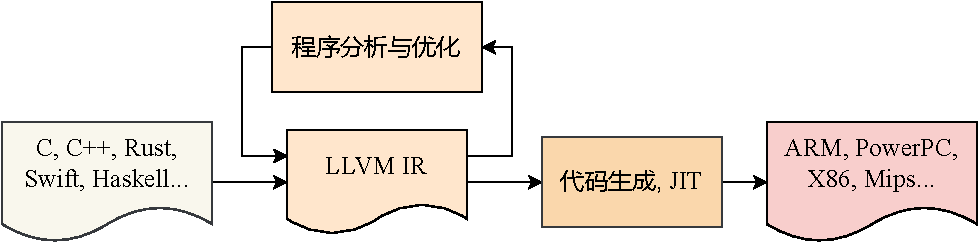
\includegraphics[width=0.8\linewidth]{figures/llvmst.pdf}
        \caption{LLVM编译框架}\label{fig:llvm}
    \end{figure}
    \item \textbf{SML-New Jersey基于LLVM编译器后端的版本:} 
    SML-New Jersey(SML/NJ)是一种经典的函数式编程语言。为了支持涌现出的各种不同的机器架构,
    SML/NJ的维护者们开发了MLRisc来作为抽象的机器层~\cite{george1994portable}。
    然而,在SML/NJ新发布的版本中,它更改了后端,将CPS中间语言编译到了LLVM IR~\cite{farvardin2020new}。
    这样的变更主要出于两种需求:为了利用LLVM编译器后端提供的丰富的分析与优化工具,以及为了支持更多的操作系统和机器架构。
    在新的SML/NJ编译器中,后端先读入高阶的CPS中间语言程序,将其转换为一阶程序,
    然后转换为控制流图(Control-Flow Graph, CFG)中间语言,再进一步转换为LLVM IR。
    使用LLVM框架之后的SML/NJ编译器生成的代码在性能上有所提升。
    但是,这项工作不是经过形式化验证的,无法保证高可靠性。
    我们的工作受到了这一趋势的启发,并进一步尝试对这种从CPS到SSA的连接进行形式化验证。
    \item \textbf{经验证的LLVM IR: Vellvm:} 
    Vellvm在定理证明工具Coq中定义了LLVM中间语言的抽象语法树(Abstract Syntax Tree, AST),并为LLVM IR提供了形式化语义。
    Vellvm还为其提供了类型系统及SSA结构相关性质的证明。
    研究者们还在Coq中实现了能够执行LLVM程序的解释器(Interpreter),来验证Vellvm的语义设计。
    利用Vellvm,我们可以将LLVM IR程序和它的Coq代码表示进行相互转换,还可以对针对LLVM IR的转换过程进行验证
    并直接插入到LLVM编译框架中。
    早期版本的Vellvm提供了LLVM IR的操作语义~\cite{zhao2012formalizing},
    而在较新版本中已迁移到了基于交互树(Interactive Tree, ITree)的语义~\cite{zakowski2021modular}。
    在本文第\ref{sec:overview}节所介绍的编译链中,SSA程序首先被编译到了Vellvm AST,然后生成了最终的LLVM IR程序。
\end{itemize}

\section{编译链概览} \label{sec:overview}

我们构建了一个从函数式语言PCF到LLVM IR的部分经过验证的编译器,并在Coq定理证明工具中
完成了编译算法和形式化验证的实现~\cite{chlipala2022certified}。
在本节中,我们主要是从高层次的角度介绍了这个编译器原型,省略了转换算法设计和证明定理的详细信息。
CPS转换及CPS到SSA转换的正确性通过源程序和目标程序之间的模拟进行形式化验证,
遵循第\ref{sec:compcertbackend}节中所介绍的CompCert后端的验证框架。
我们使用$\approx $表示语义保存性质。PCF、CPS和SSA的程序分别表示为$t_{pcf}$、$t_{cps}$和$t_{ssa}$。
通过对$t_{pcf}\approx t_{cps}$和$t_{cps}\approx t_{ssa}$的形式化证明,可以组合推导出$t_{pcf}\approx t_{ssa}$。
然后我们就得到了一个从PCF到SSA的经验证的编译过程。我们应用该经验证的编译过程,构建出一个编译器原型。
该编译器读取PCF程序,并经过图\ref{overview}中所示的几个编译步骤生成LLVM IR程序。

\begin{figure}[htbp]
    \centering
    \vspace{2ex}
    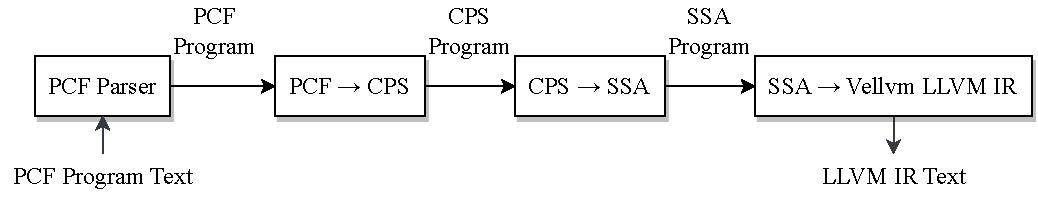
\includegraphics[width=0.8\linewidth]{figures/overview.pdf}
    \caption{PCF到LLVM编译链概览}\label{overview}
\end{figure}

\subsection{读入PCF文本}

使用PCF语法分析器(Parser)将文本形式的PCF程序提取为Coq中的结构化PCF代码项。
为了分析文本信息并提取PCF程序,获取源程序的语法结构至关重要。对于文本形式的PCF程序,
我们首先用词法分析器(Lexical Parser)将其解析为令牌(Token)流。
随后,使用语法分析器(Syntax Parser)分析该令牌流,生成Coq中的直接风格PCF程序项的抽象语法树。

\subsection{CPS转换}

如第\ref{sec:background}节中所言,函数式编程语言的编译器通常会将直接风格的程序转换为CPS形式,以获得显式的控制流。
我们已经得到了PCF程序的抽象语法树,但它是直接风格的程序,所以接下来需要使用CPS转换将其编译为CPS风格的程序。
将直接风格的PCF程序转换为CPS形式的算法主要由当前代码项和当前项被规约为某个值后要处理的下一个项决定。
另外,我们为直接风格及CPS风格的PCF语言定义了小步操作语义,并证明了CPS转换的前向模拟性质。
关于该CPS转换算法及其正确性验证的详细信息将在第\ref{sec:cpstrans}节和第\ref{sec:cpsforward}节中进行讨论。

\subsection{从CPS到SSA}

该编译链中最关键的部分是从CPS风格的函数式程序到目标SSA程序的转换及验证。
目标SSA语言是LLVM IR的简化版本,保留了其最基本的结构和程序语句。
通过该编译过程,输入的CPS程序项将被转换为一个包含主函数的SSA程序。
同样的,我们为这种SSA语言定义了小步操作语义,并证明了从CPS到SSA转换的前向模拟。
完成这一步证明后,我们将正向模拟组合起来,并完成了从源程序到SSA程序后向模拟的证明。
在第\ref{sec:cpsssatrans}节中将详细介绍该转换算法的设计和细节。
第\ref{sec:cpsssaforward}节中将进行CPS到SSA转换算法的形式化验证,并通过运行一个示例程序展示前向模拟的每一个关键步骤。

\subsection{从SSA到LLVM IR}

上一步中得到的SSA程序被转换为Vellvm中的抽象语法树,然后转换为LLVM IR程序文本。
在该编译链中,我们使用了经过验证的LLVM基础设施Vellvm~\cite{zakowski2021modular}。
利用其在Coq实现的LLVM IR的抽象语法树,我们可以进一步输出最终的LLVM IR程序。
由于我们使用的SSA语言是LLVM IR的简化版本,它保留了LLVM IR程序的基本结构,
可以方便地编译到Vellvm中的抽象语法树。这种SSA语言省略了LLVM IR中的大部分参数。
例如,函数定义在LLVM中非常复杂,有很多可选的参数,而本文中的SSA语言只保留了函数定义中必须指定的内容。
LLVM中的表达式类型多种多样,其中整数包括多种宽度的i16、i32等,
而本文的SSA语言简化为没有明确指定类型的无限宽自然数。
该编译过程的主要工作其实就是为这些被省略的参数选取正确的默认值。
